\documentclass[17pt, a0paper, portrait]{tikzposter}
\usepackage[utf8]{inputenc}

%% Further useful packages (included in most LaTeX distributions)
\usepackage{amsmath}        % extensions for typesetting of math
\usepackage{amsfonts}       % math fonts
\usepackage{amsthm}         % theorems, definitions, etc.
\usepackage{bbding}         % various symbols (squares, asterisks, scissors, ...)
\usepackage{bm}             % boldface symbols (\bm)
\usepackage{graphicx}       % embedding of pictures
\usepackage{fancyvrb}       % improved verbatim environment
\usepackage{natbib}         % citation style AUTHOR (YEAR), or AUTHOR [NUMBER]
\usepackage{dcolumn}        % improved alignment of table columns
\usepackage{booktabs}       % improved horizontal lines in tables
\usepackage{paralist}       % improved enumerate and itemize

\usepackage{algorithm}
\usepackage{algpseudocode}
\usepackage{mathtools}
\usepackage[acronym,toc]{glossaries}

% poster specific
\usepackage{blindtext}
\usepackage{comment}
\usepackage{lmodern}

%%% Basic information on the thesis

% Thesis title in English (exactly as in the formal assignment)
\def\ThesisTitle{Map-merging for multi-robot system}

% Author of the thesis
\def\ThesisAuthor{Jiří Hörner}

% Year when the thesis is submitted
\def\YearSubmitted{2016}

% Name of the department or institute, where the work was officially assigned
% (according to the Organizational Structure of MFF UK in English,
% or a full name of a department outside MFF)
\def\Department{Department of Theoretical Computer Science and Mathematical Logic}

% Is it a department (katedra), or an institute (ústav)?
\def\DeptType{Department}

% Thesis supervisor: name, surname and titles
\def\Supervisor{RNDr. David Obdržálek, Ph.D.}

% Supervisor's department (again according to Organizational structure of MFF)
\def\SupervisorsDepartment{Department of Theoretical Computer Science and Mathematical Logic}

% Study programme and specialization
\def\StudyProgramme{Computer Science}
\def\StudyBranch{General Computer Science}

% An optional dedication: you can thank whomever you wish (your supervisor,
% consultant, a person who lent the software, etc.)
\def\Dedication{%
I acknowledge my colleague Lukas Jelinek for sharing his insights into VREP simulator. I wish to thank to my family for support.
}

% Abstract (recommended length around 80-200 words; this is not a copy of your thesis assignment!)
\def\Abstract{%
A set of robots mapping an area can potentially combine their information to produce a distributed map more efficiently and reliably than a single robot alone. Multi-robot swarm coordination depends on a consistent, reliable map of the environment. Map-merging algorithms are therefore key komponents for such systems. In this work I present a novel algorithm for merging two-dimensinal maps created by different robots independently without initial knowledge of relative poses of robots. The algorithm is inspired by computer vision image stitching techniques for creating photo panoramas. Presented algorithm relies only on map data represented as occupancy grids, which allows great scalabity for heterogeneous multi-robot swarms and makes algorithm easily deployable with various \gls{SLAM} algorithms. The map-merging algorithm was implemented as publicily available \gls{ROS} package and was accepted in \gls{ROS} distribution. Performance of the algorithm has been evaluated in \gls{ROS} enviroment using \gls{VREP} simulator. For purposes of evaluation \gls{ROS} package for exploring was developed as part of this work.
}

% 3 to 5 keywords (recommended), each enclosed in curly braces
\def\Keywords{%
{map-merging} {multi-robot system} {ROS} {SLAM} {image stitching}
}

%%% This file contains definitions of various useful macros and environments %%%
%%% Please add more macros here instead of cluttering other files with them. %%%

%%% Minor tweaks of style

% These macros employ a little dirty trick to convince LaTeX to typeset
% chapter headings sanely, without lots of empty space above them.
% Feel free to ignore.
\makeatletter
\def\@makechapterhead#1{
  {\parindent \z@ \raggedright \normalfont
   \Huge\bfseries \thechapter. #1
   \par\nobreak
   \vskip 20\p@
}}
\def\@makeschapterhead#1{
  {\parindent \z@ \raggedright \normalfont
   \Huge\bfseries #1
   \par\nobreak
   \vskip 20\p@
}}
\makeatother

% This macro defines a chapter, which is not numbered, but is included
% in the table of contents.
\def\chapwithtoc#1{
\chapter*{#1}
\addcontentsline{toc}{chapter}{#1}
}

% Draw black "slugs" whenever a line overflows, so that we can spot it easily.
\overfullrule=1mm

%%% Macros for definitions, theorems, claims, examples, ... (requires amsthm package)

\theoremstyle{plain}
\newtheorem{thm}{Theorem}
\newtheorem{lemma}[thm]{Lemma}
\newtheorem{claim}[thm]{Claim}

\theoremstyle{plain}
\newtheorem{defn}{Definition}

\theoremstyle{remark}
\newtheorem*{cor}{Corollary}
\newtheorem*{rem}{Remark}
\newtheorem*{example}{Example}

%%% An environment for proofs

%%% FIXME %%% \newenvironment{proof}{
%%% FIXME %%%   \par\medskip\noindent
%%% FIXME %%%   \textit{Proof}.
%%% FIXME %%% }{
%%% FIXME %%% \newline
%%% FIXME %%% \rightline{$\square$}  % or \SquareCastShadowBottomRight from bbding package
%%% FIXME %%% }

%%% An environment for typesetting of program code and input/output
%%% of programs. (Requires the fancyvrb package -- fancy verbatim.)

\DefineVerbatimEnvironment{code}{Verbatim}{fontsize=\small, frame=single}

%%% The field of all real and natural numbers
\newcommand{\R}{\mathbb{R}}
\newcommand{\N}{\mathbb{N}}

%%% Useful operators for statistics and probability
\DeclareMathOperator{\pr}{\textsf{P}}
\DeclareMathOperator{\E}{\textsf{E}\,}
\DeclareMathOperator{\var}{\textrm{var}}
\DeclareMathOperator{\sd}{\textrm{sd}}

%%% Transposition of a vector/matrix
\newcommand{\T}[1]{#1^\top}

%%% Various math goodies
\newcommand{\goto}{\rightarrow}
\newcommand{\gotop}{\stackrel{P}{\longrightarrow}}
\newcommand{\maon}[1]{o(n^{#1})}
\newcommand{\abs}[1]{\left|{#1}\right|}
\newcommand{\dint}{\int_0^\tau\!\!\int_0^\tau}
\newcommand{\isqr}[1]{\frac{1}{\sqrt{#1}}}

%%% Various table goodies
\newcommand{\pulrad}[1]{\raisebox{1.5ex}[0pt]{#1}}
\newcommand{\mc}[1]{\multicolumn{1}{c}{#1}}

%%% My macros

\DeclareMathOperator{\rank}{rank}
\DeclareMathOperator{\sgn}{sgn}
\DeclareMathOperator{\trace}{trace}
\DeclareMathOperator{\conv}{conv}
%\DeclareMathOperator{\R}{\mathbb{R}}
\DeclareMathOperator{\bigO}{\mathcal{O}}
\DeclarePairedDelimiter{\ev}{\operatorname{E}[}{]}
\DeclarePairedDelimiter{\prob}{\operatorname{P}[}{]}
%\DeclarePairedDelimiter{\abs}{\lvert}{\rvert}
\DeclarePairedDelimiter{\ceil}{\lceil}{\rceil}
\DeclarePairedDelimiter{\floor}{\lfloor}{\rfloor}
\DeclarePairedDelimiter{\norm}{\lVert}{\rVert}
\DeclarePairedDelimiter{\scal}{\langle}{\rangle}

\renewcommand{\algorithmicrequire}{\textbf{Input:}}
\renewcommand{\algorithmicensure}{\textbf{Output:}}

% ROS node API formatting
\newcommand{\ROStopic}[3]{\begin{sloppypar} \noindent\texttt{#1} (#2) \end{sloppypar} \par \hangindent=15pt \hangafter=0 \noindent #3}
\newcommand{\ROSparam}[4]{\begin{sloppypar} \noindent\texttt{#1} (#3, default: \texttt{#2}) \end{sloppypar} \par \hangindent=15pt \hangafter=0 \noindent #4}
\newcommand{\ROStransform}[3]{\begin{sloppypar} \noindent\texttt{#1} $\rightarrow$ \texttt{#2} \end{sloppypar} \par \hangindent=15pt \hangafter=0 \noindent #3}

% allow hyphenation after underscore
\let\oldunderscore\_
\renewcommand{\_}{\oldunderscore\-}

\hyphenation{mer-ged}

%%% Abbreviations used in the thesis, if any, including their explanation

\newacronym{RANSAC}{RANSAC}{random sample consensus}
\newacronym{BFS}{BFS}{breadth-first search}
\newacronym{DFS}{DFS}{depth-first search}
\newacronym{ROS}{ROS}{Robot Operating System}
\newacronym{OpenCV}{OpenCV}{Open Source Computer Vision Library}
\newacronym{ORB}{ORB}{Oriented FAST and Rotated BRIEF}
\newacronym{SIFT}{SIFT}{scale-invariant feature transform}
\newacronym{SURF}{SURF}{Speeded Up Robust Features}
\newacronym{SLAM}{SLAM}{simultaneous localization and mapping}
\newacronym{FLANN}{FLANN}{Fast Library for Approximate Nearest Neighbors}
\newacronym{SIG}{SIG}{Special Interest Group}

% poster styling

% university color style
\definecolorstyle{UKColorStyle}{
    % Define default colors
    % university red used in logo text
    % \definecolor{colorOne}{HTML}{D62153}
    \definecolor{colorOne}{cmyk}{0.1484,1,0.6729,0.0548}
    % \definespotcolor{colorOne}{PANTONE 193 C}{0.14,1,0.66,0.03}
    % \definecolor{colorOne}{cmyk}{0.14,1,0.66,0.03}
    % \definecolor{colorOne}{RGB}{133,53,47}
    % \definecolor{colorOne}{RGB}{198,9,59}
    % nice gray
    \definecolor{colorTwo}{HTML}{CCCCCC}
    % university official red for logo
    \definecolor{colorThree}{cmyk}{0,0.91,0.65,0.11}
}{
    % Background Colors
    \colorlet{backgroundcolor}{white}
    \colorlet{framecolor}{colorTwo}
    % Title Colors
    \colorlet{titlefgcolor}{black}
    \colorlet{titlebgcolor}{white}
    % Block Colors
    \colorlet{blocktitlefgcolor}{white}
    \colorlet{blocktitlebgcolor}{colorOne}
    \colorlet{blockbodyfgcolor}{black}
    \colorlet{blockbodybgcolor}{white}
    % Innerblock Colors
    \colorlet{innerblocktitlebgcolor}{colorThree}
    \colorlet{innerblocktitlefgcolor}{white}
    \colorlet{innerblockbodybgcolor}{white}
    \colorlet{innerblockbodyfgcolor}{black}
    % Note colors
    \colorlet{notefgcolor}{black}
    \colorlet{notebgcolor}{colorThree!40!white}
    \colorlet{notefrcolor}{colorThree!40!white}
 } % space is important here

\definetitlestyle{FilledWithBottomLine}{
    width=\paperwidth, roundedcorners=0, linewidth=0pt, innersep=1.5cm,
    titletotopverticalspace=0mm, titletoblockverticalspace=20mm,
    titlegraphictotitledistance=10pt
}{
    \draw[draw=none, fill=titlebgcolor]%
    (\titleposleft,\titleposbottom) rectangle (\titleposright,\titlepostop); %
    \draw[draw=none, fill=colorOne]%
    (\titleposleft,\titleposbottom+40) rectangle (\titleposright,\titleposbottom); %
}

% theme for our university, created by me
% aligned with university graphical manual
\definelayouttheme{Charles}{
    \usecolorstyle{UKColorStyle}
    \usebackgroundstyle{Default}
    \usetitlestyle{FilledWithBottomLine}
    \useblockstyle{Basic}
    \useinnerblockstyle{Default}
    \usenotestyle{VerticalShading}
}

% custom title with logo at the left
\makeatletter
\renewcommand\TP@maketitle{%
    \begin{minipage}{0.25\linewidth}
       \centering
       \@titlegraphic
    \end{minipage}
    \hfill
    \begin{minipage}{0.75\linewidth}
        \centering
        \color{titlefgcolor}
        % {\bfseries \Huge \sc \@title \par}
        {\fontsize{50}{60} \bfseries \@title \par}
        % {\Huge \bfseries \@title \par}
        \vspace*{1.5em}
        {\Huge \@author \par}
        \vspace*{1.5em}
        {\LARGE \@institute}
    \end{minipage}%
    \vspace{40pt}
}
\makeatother

% fix bug with algorithm envirinment
\AtBeginEnvironment{algorithm}{%
  \setlength{\columnwidth}{\linewidth}%
}

% blocks with emphasis (different color)
\newenvironment{blockemph}
{
    \begin{@empty}
    \colorlet{blocktitlefgcolor}{colorOne}
    \colorlet{blocktitlebgcolor}{white}
    \colorlet{framecolor}{colorOne}
}{
    \end{@empty}
}


\usetheme{Charles}

\title{\ThesisTitle}
\author{\ThesisAuthor}
\date{\YearSubmitted}
\institute{\Department}
\titlegraphic{
\includegraphics[height=15em]{../img/logotyp_fakulty2.pdf}}

\begin{document}

\maketitle

% \block{~}
% {
%     \Abstract
% }

\begin{columns}
\column{0.25}
\block{Merging algorithm}{
\begin{tikzfigure}[\gls{OpenCV} Stitching pipeline.]
    \centering
    % 4.33in for 300 dpi
    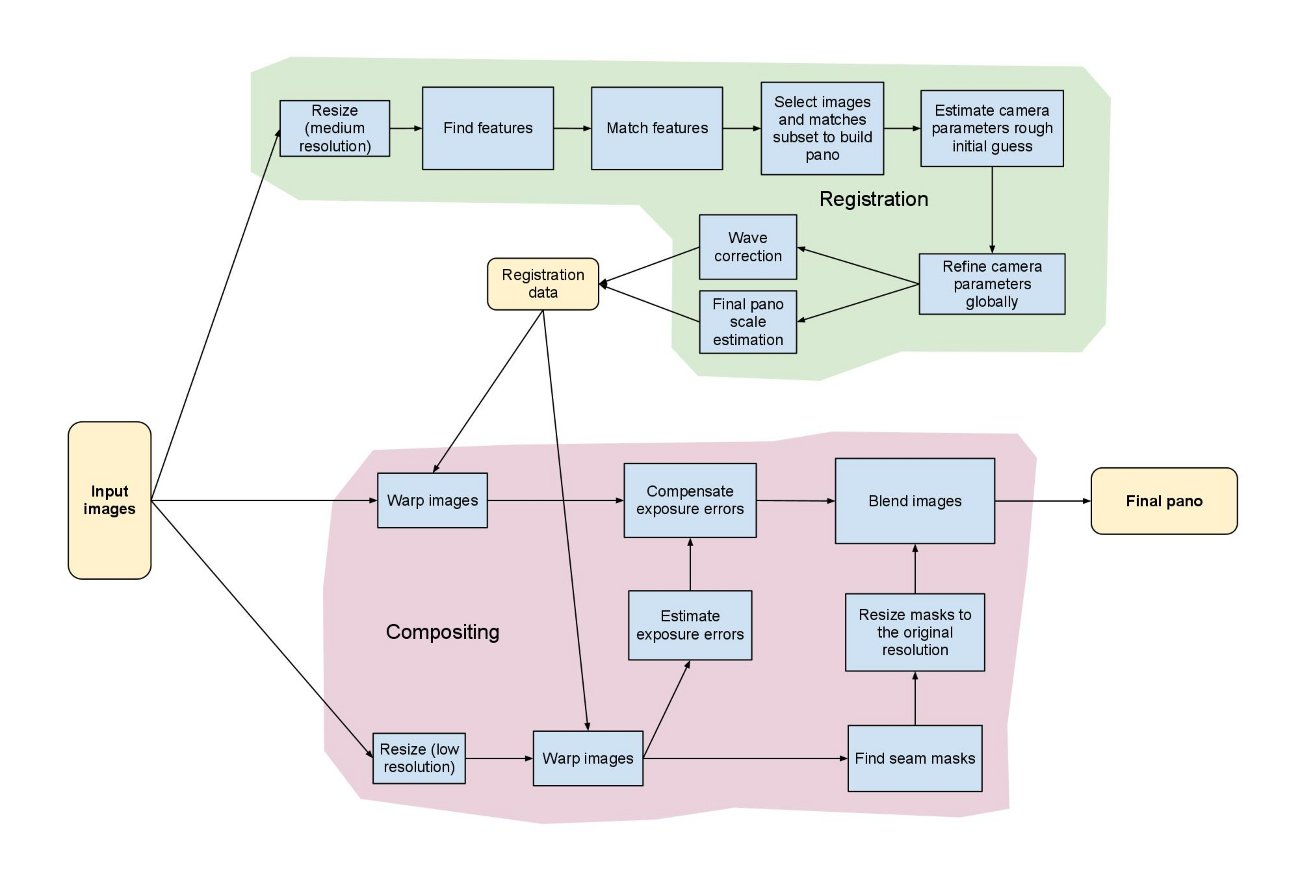
\includegraphics[width=\linewidth]{../img/StitchingPipeline.jpg}
    \label{fig:opencv}
\end{tikzfigure}


\begin{algorithm}[H]
    \caption{Proposed algorithm for estimating transformation between multiple occupancy grids. Uses Algorithm~\ref{alg:estimatefinaltrans} to estimate final transformations.}
    \label{alg:estimategridtrasform}
    \begin{algorithmic}[1]
        \Require $k$ occupancy grids
        \Ensure for each grid: transformation between grid and global reference frame, or value indicating transformation could not be be estimated for current grid
        \Procedure{estimateGridTransform}{$grids$}
            \State detect \gls{ORB} features (keypoints) for each grid
            \ForAll{$(i,j)$ pair of grids} \Comment{compute transform for each pair}
                \State match features
                \State $n \gets \text{number of matches}$
                \If{$n \le \text{matches threshold}$}
                    \State confidence $\gets 0$
                \Else
                    \State try find restricted affine transformation for features with \gls{RANSAC}
                    \State $\psi \gets \text{number of inliers in \gls{RANSAC}}$
                    \If{transformation found}
                        \State confidence $\gets \frac{\psi}{8 + 0.3 \cdot n}$
                        \State $P_{(i,j)} \gets$ restricted affine transformation
                    \Else
                        \State confidence $\gets 0$
                    \EndIf
                \EndIf
            \EndFor
            \State matches $\gets (i,j)$ for matches with confidence $\ge 1.0$
            \State $g \gets (grids, matches)$
            \State $h \gets$ largest connected component in $g$
            \State $t \gets$ maximum spanning tree in $h$
            \State \Call{estimateFinalTransform}{$t$, $P_{(i,j)} \forall e \in \text{edges of } t$} \Comment{walk $t$ and compute transformations to global reference frame. See Algorithm~\ref{alg:estimatefinaltrans}.}
        \EndProcedure
    \end{algorithmic}
\end{algorithm}


\begin{tikzfigure}[Graph showing matches between $36$ occupancy grids during map merging. Legend: $Nm$ number of matches, $Ni$ number of inliers from \gls{RANSAC}, $C$ confidence.]
    \centering
    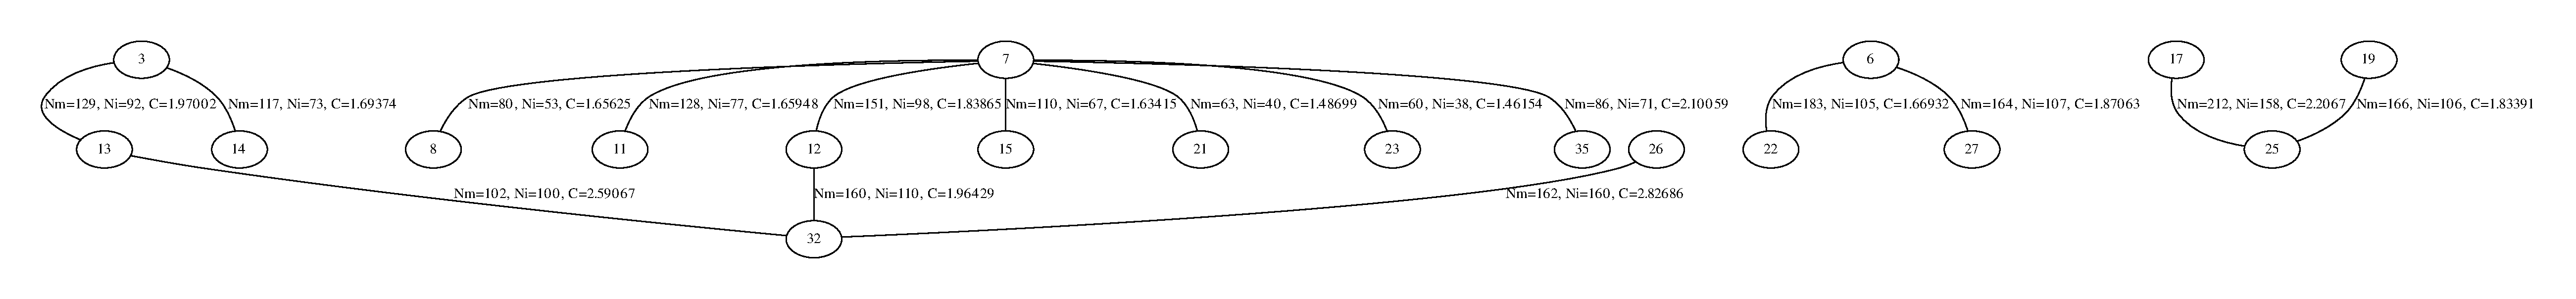
\includegraphics[width=\linewidth]{../img/matches.pdf}
    \label{fig:matches}
\end{tikzfigure}


\begin{defn}[Reduced affine transformation]
For given matrices $R$ (rotation), $S$ (scaling), $T$ (translation), where
\begin{align}
    R &=
    \begin{pmatrix}
        \cos{\theta} & -\sin{\theta} \\
        \sin{\theta} & \cos{\theta} \\
    \end{pmatrix} \\
    S &=
    \begin{pmatrix}
        s & 0 \\
        0 & s \\
    \end{pmatrix} \\
    T &=
    \begin{pmatrix}
        tx \\
        ty \\
    \end{pmatrix}
\end{align}
we define matrix of reduced affine transformation as
\begin{equation}
    A =
    \begin{pmatrix}
        RS|T
    \end{pmatrix}
    =
    \begin{pmatrix}
        \cos(\theta)s & -\sin(\theta)s & tx \\
        \sin(\theta)s & \cos(\theta)s & ty \\
    \end{pmatrix}
\end{equation}
\end{defn}

We need to solve~\eqref{eq:affinetrans} to estimate reduced affine trasformation between grids.
\begin{align}
    A'X &= Y \label{eq:affinetrans}\\
    \begin{pmatrix}
        \cos(\theta)s & -\sin(\theta)s & tx \\
        \sin(\theta)s & \cos(\theta)s & ty \\
        0 & 0 & 1 \\
    \end{pmatrix}
    \begin{pmatrix}
        x_1 \\
        x_2 \\
        1
    \end{pmatrix}
    &=
    \begin{pmatrix}
        y_1 \\
        y_2 \\
        1
    \end{pmatrix}
\end{align}


\begin{algorithm}[H]
    \caption{Algorithm estimating transformations to global reference frame from pairwise transformations on spanning tree.}
    \label{alg:estimatefinaltrans}
    \begin{algorithmic}[1]
        \Require $t$ maximum spanning tree on grids, $P_{(i,j)}$ pairwise reduced affine transformation in homogeneous coordinates between grids $i, j$.
        \Ensure $T_i \forall i \in V$ transformations to global reference frame
        \Procedure{estimateFinalTransform}{$t = (V,E)$, $P_e \forall e \in e$}
            \State $e \gets$ edges of $t$ sorted by discover time in \gls{BFS} starting from grid with global reference frame \Comment{using \gls{BFS} or \gls{DFS} does not matter here}
            \State $\forall T_i: T_i \gets I$ \Comment{initialize transformations with identity}
            \ForAll{$(i,j)$ in $e$}
                $T_j \gets T_i P_{(i,j)}$
            \EndFor
        \EndProcedure
    \end{algorithmic}
\end{algorithm}
} % end block

\column{0.5}
\block{Merging with unknown initial positions}{
\begin{minipage}[t]{0.47\linewidth}
    \begin{tikzfigure}[Maps produced by a multi-robot mapping in the simulator with $3$ robots. The merged map (bottom right) is estimated by the map-merging node without knowledge of initial positions.]
        \centering
        % 2.22in for 300dpi
        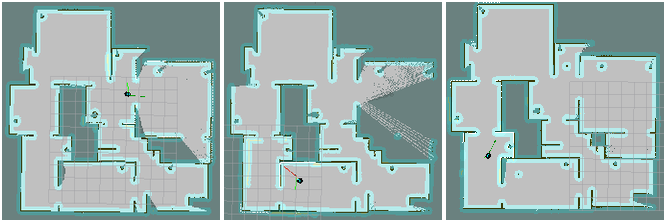
\includegraphics[width=\linewidth]{../img/minimal-overlapping-area-final-maps.png}
        \label{fig:minimal-overlapping-area-final-maps}
    \end{tikzfigure}
\end{minipage}
\hfill
\begin{minipage}[t]{0.47\linewidth}
    \begin{tikzfigure}[Excerpt from the attached log of the map-merging node captured during simulation. Shows output of matching phase of the algorithm for $3$ pairwise matches along with number of inliers.]
        \VerbatimInput[fontsize=\small, frame=single]{../img/log-excerpt.txt}
        ~ % this is important
    \end{tikzfigure}
\end{minipage}
} % end block

\block{Merging with known initial positions}{
\begin{minipage}[t]{0.47\linewidth}
    \begin{tikzfigure}[Initial maps produced by robots during experiment in the simulator. Merged map is produced with knowledge of initial positions and can be therefore produced even without overlapping areas. In this situation merged map can be sparse.]
        \centering
        % 3.35in
        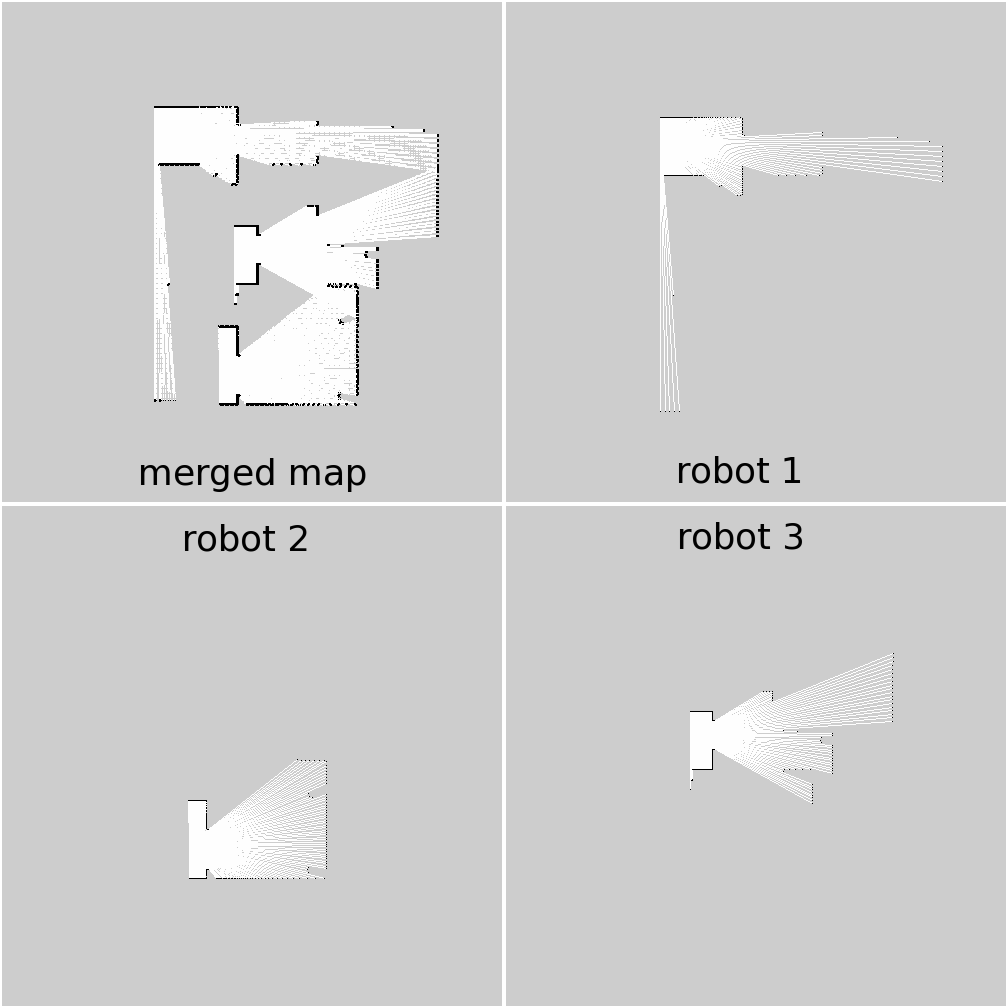
\includegraphics[width=\linewidth]{../img/merging-with-known-initial-positions-begin.png}
        \label{fig:merging-with-known-initial-positions-begin}
    \end{tikzfigure}
\end{minipage}
\hfill
\begin{minipage}[t]{0.47\linewidth}
    \begin{tikzfigure}[Final maps produced in the simulator. Merged map is produced with knowledge of initial positions.]
        \centering
        % 3.35in for 300 dpi
        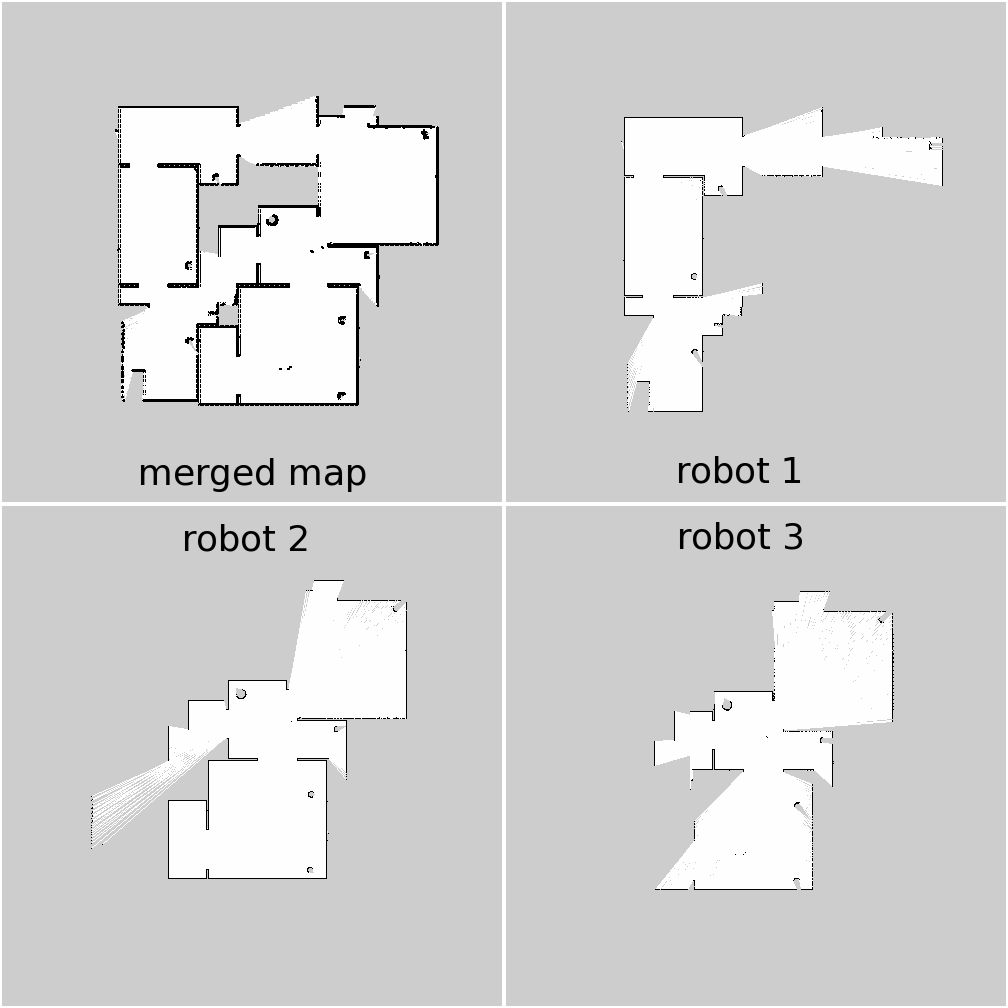
\includegraphics[width=\linewidth]{../img/merging-with-known-initial-positions-end.png}
        \label{fig:merging-with-known-initial-positions-end}
    \end{tikzfigure}
\end{minipage}
} % end block

\block{Rejecting maps with errors}{
\begin{minipage}[t]{0.47\linewidth}
    \begin{tikzfigure}[$36$ maps created by \texttt{hector\_slam} from \gls{MIT} dataset. Note that the most of the maps contain serious mapping errors. These errors usually come from \gls{SLAM} invalid estimation of rotation, generating misaligned walls and corners. Because of the new walls and corners, broken maps tend to have more features, especially in broken areas, making filtering of broken maps hard.]
        \centering
        \includegraphics[width=\linewidth]{../img/mit-dataset-montage.png}
        \label{fig:probability-model-evaluation-montage}
    \end{tikzfigure}
\end{minipage}
\hfill
\begin{minipage}[t]{0.47\linewidth}
    \begin{tikzfigure}[Merged map. All broken maps have been rejected by probalistic model used by merging algorithm. The merged map is correct, transformation between grids was estimated correctly. Maps included in this merged map are small, for larger maps the \gls{SLAM} algorithm mostly failed on presented dataset. Only $3$ maps are included in the merged map. Confidence threshold is set to $2.0$.]
        \centering
        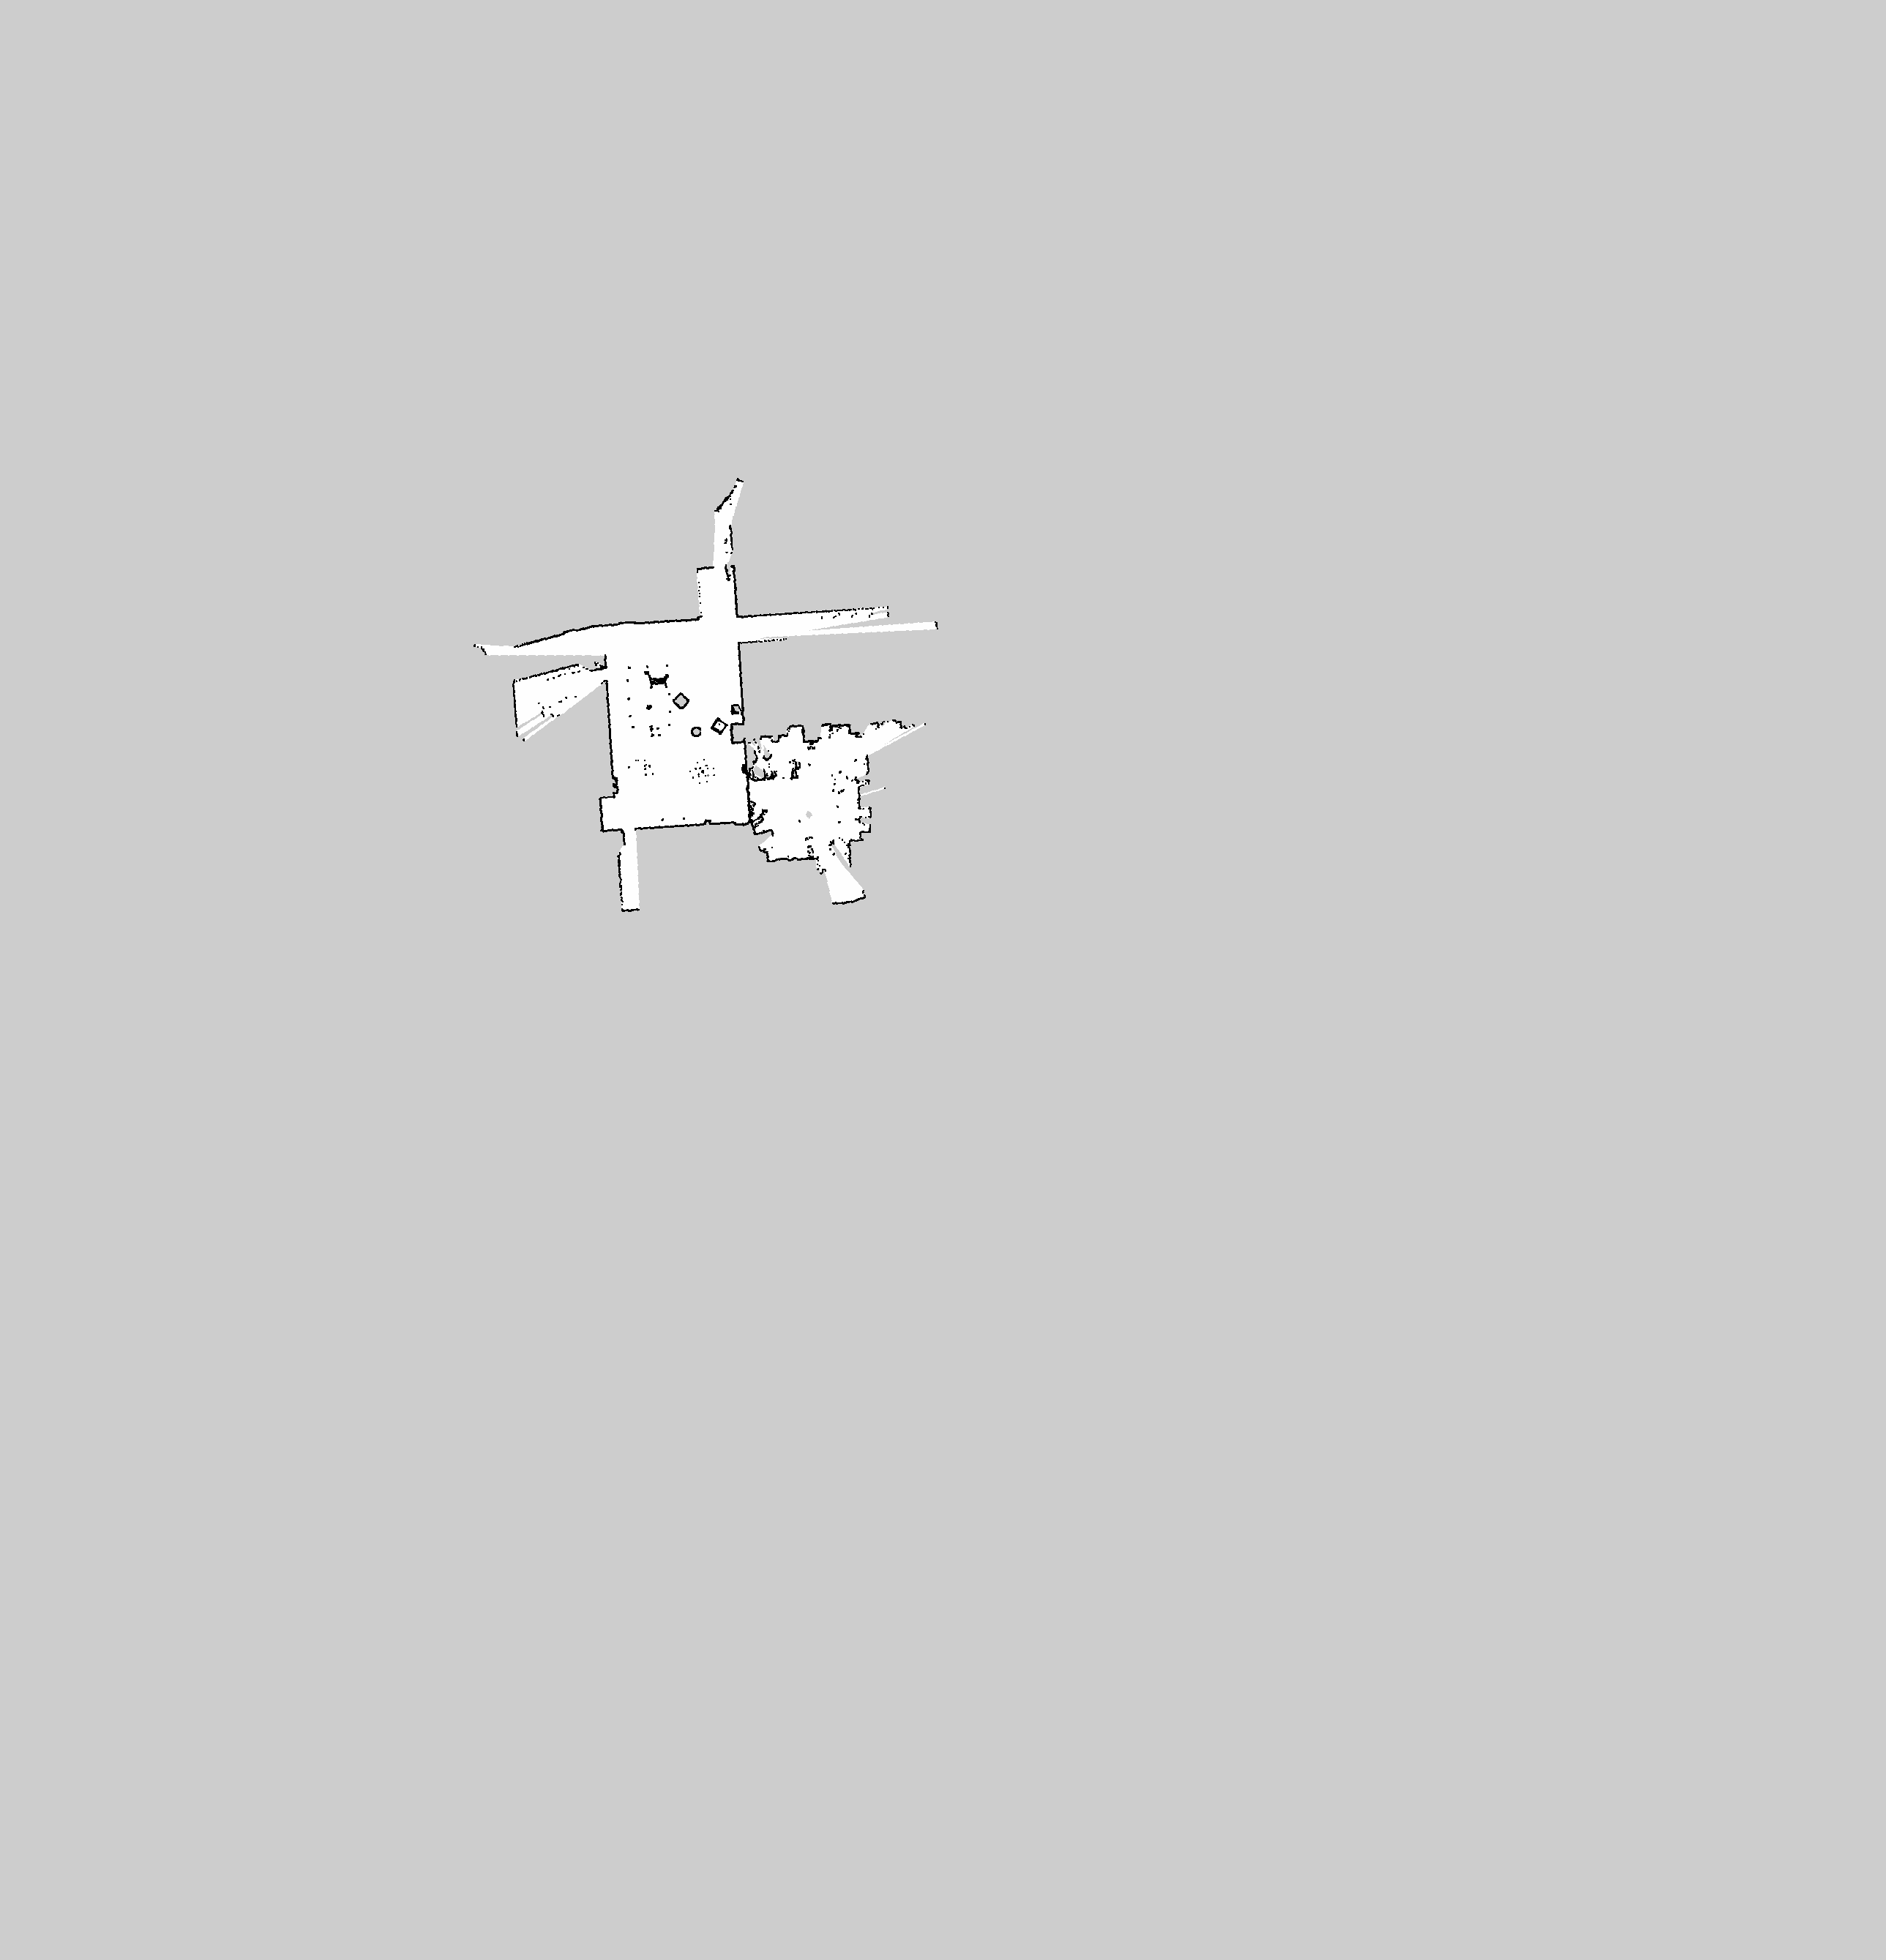
\includegraphics[width=\linewidth]{../img/probability-model-evaluation-treshold_2_0-3maps.png}
        \label{fig:probability-model-evaluation-treshold_2.0-3maps}
\end{tikzfigure}
\end{minipage}
} % end block

\block{Retaining largest transformation}{
\begin{tikzfigure}[Map-merging with largest transformation retaining. From the left: Maps have no overlaps, unable to merge more than a single map. Incorrect transformation estimated due to too small overlaps. Overlapping space is still too small to produce a merge, but incorrect transformation was rejected. Due to largest transformation retaining incorrect merge is still produced.]
    \centering
    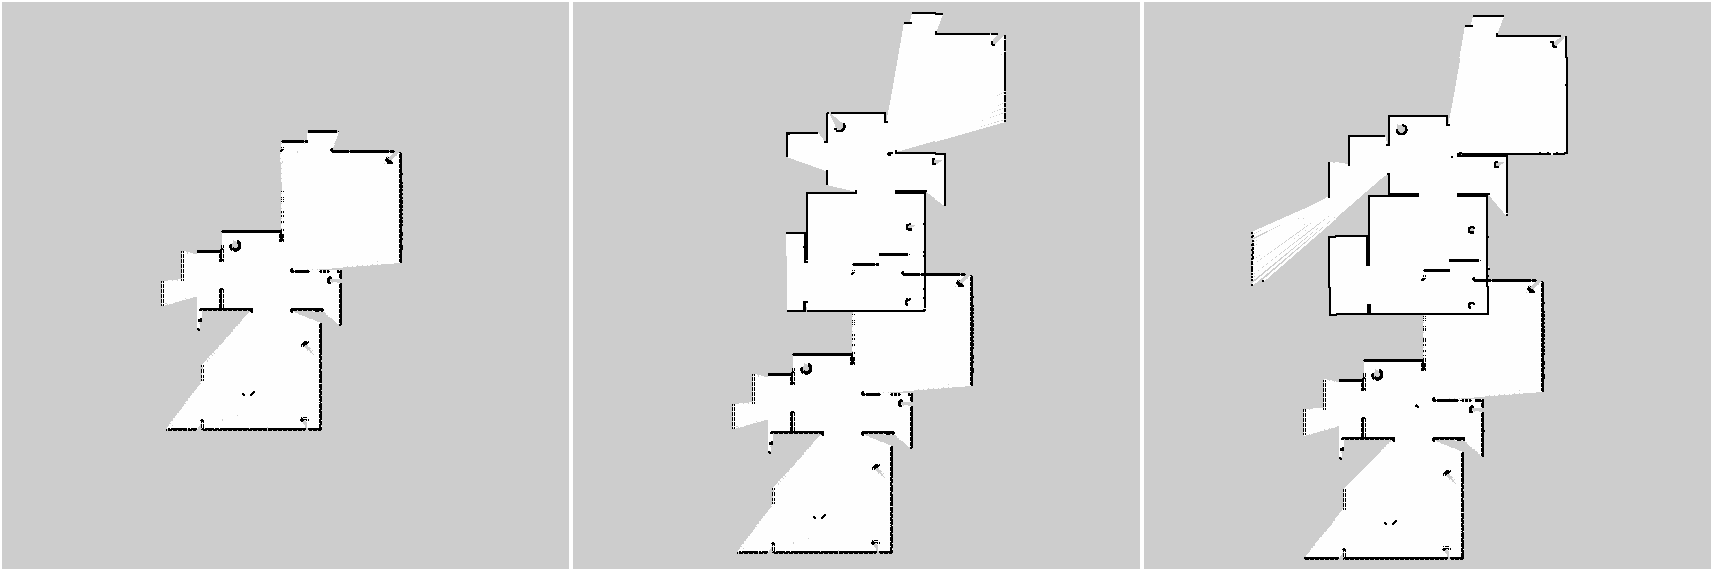
\includegraphics[width=\linewidth]{../img/retaining-largest-transformation-montage.png}
    \label{fig:retaining-largest-transformation-montage}
\end{tikzfigure}
} % end block

\column{0.25}
\block{\gls{ROS} packages}{\blindtext \vspace{4cm}
\note[
    targetoffsetx=0cm,
    targetoffsety=0cm,
    width=\linewidth
    ]
{e-mail \texttt{me@nirvana.com}}
} % end block

\block{Simulation}{
\begin{tikzfigure}[Scene for experiment with $3$ robots in \gls{VREP} simulator. Robot positions in scene are used as initial positions of robots for experiment.]
    \centering
    % orig width 3.93in
    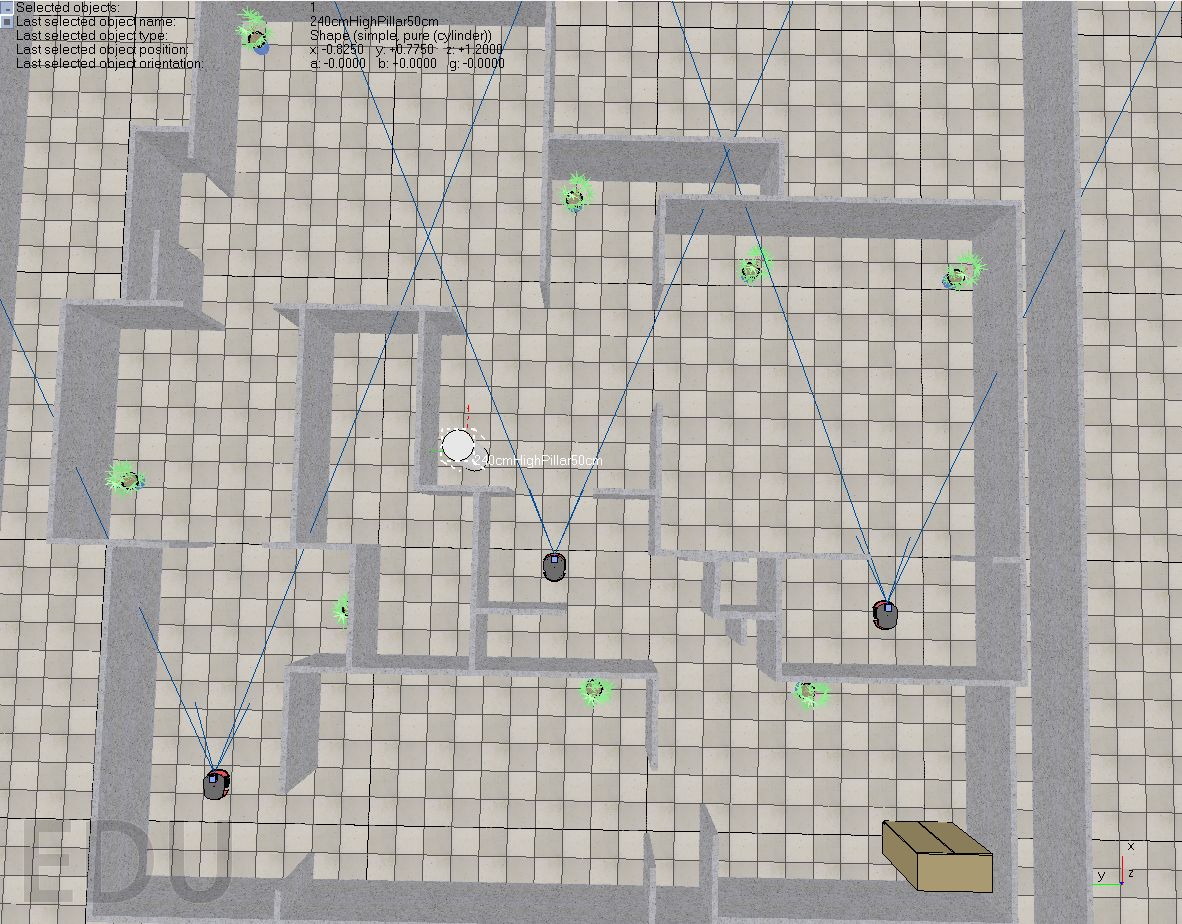
\includegraphics[width=\linewidth]{../img/minimal-overlapping-area-scene.png}
    \label{fig:minimal-overlapping-area-scene}
\end{tikzfigure}
} % end block

\block{multirobot\_map\_merge}{
Map-merging node for \gls{ROS}.
\begin{tikzfigure}[Output of \texttt{multirobot\_map\_merge}, map merging node for \gls{ROS}. The merged map for $2$ robots. Robots in the environment visualised on the left, merged map on the right.]
    \centering
    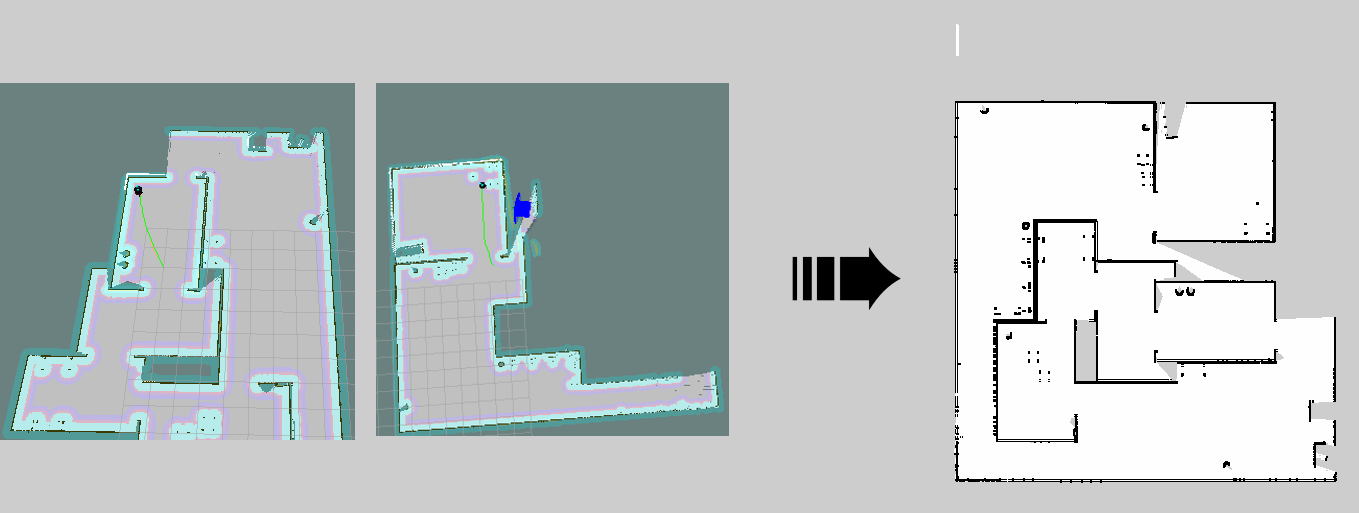
\includegraphics[width=4.53in]{../img/map_merge_cover.png}
    \label{fig:mapmergecover}
\end{tikzfigure}

\begin{tikzfigure}[Architecture of \texttt{multirobot\_map\_merge}.]
    \centering
    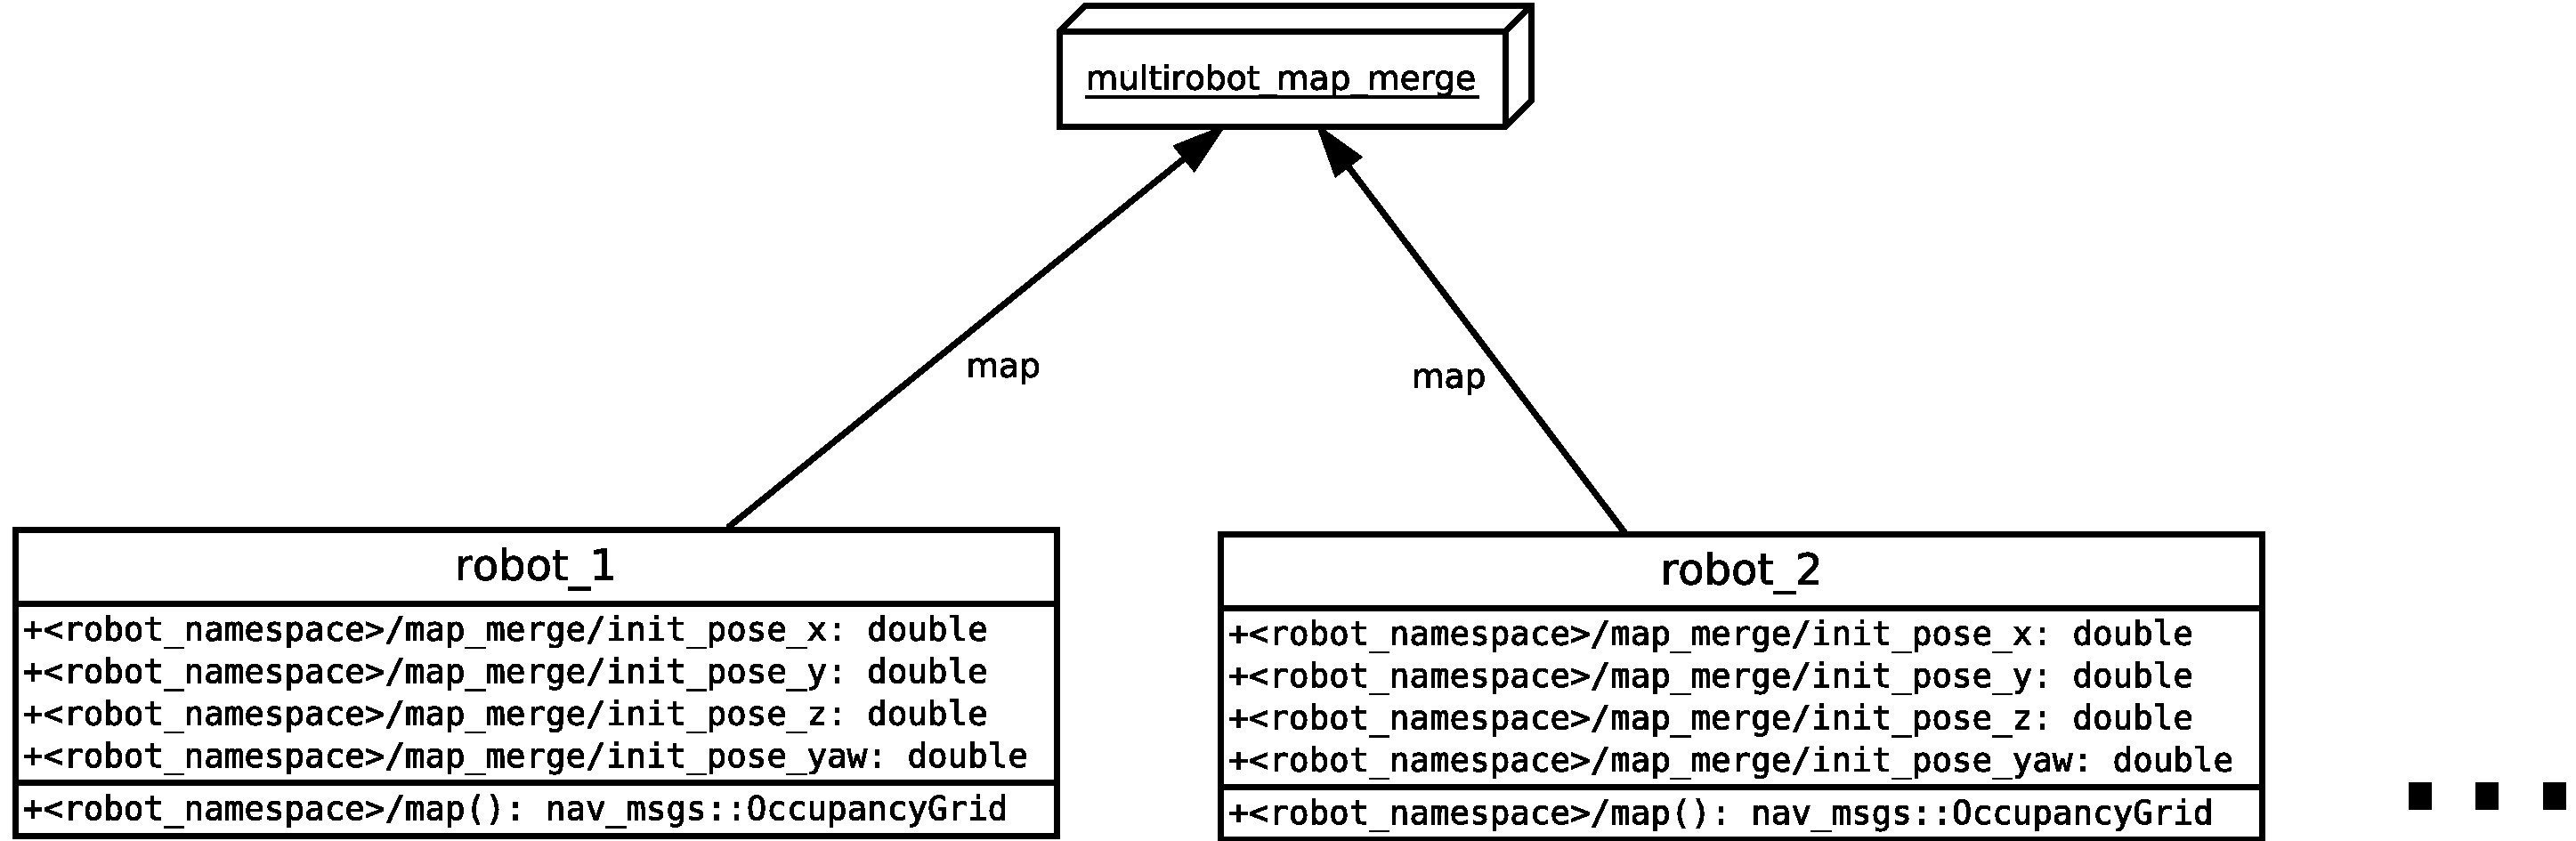
\includegraphics[width=\linewidth]{../img/map_merge_architecture.pdf}
    \label{fig:mapmergearchitecture}
\end{tikzfigure}
} % end block

\block{explore\_lite}{
\gls{ROS} node autonomous exploring.
\begin{tikzfigure}[Visualisation of robot during exploring.]
    \centering
    % orig width 2.68in
    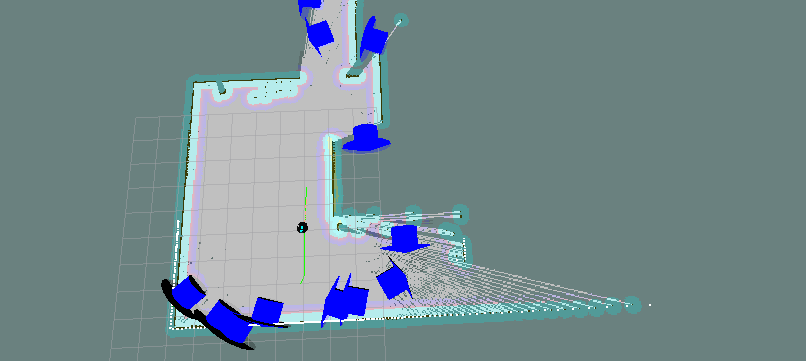
\includegraphics[width=\linewidth]{../img/explore_cover.png}
    \label{fig:explorecover}
\end{tikzfigure}

\begin{tikzfigure}[Architecture of \texttt{explore\_lite}]
    \centering
    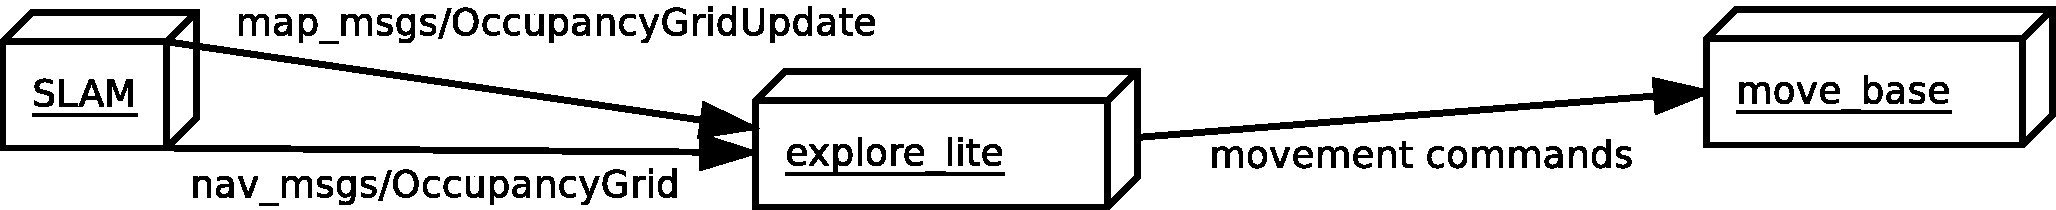
\includegraphics[width=\linewidth]{../img/explore_architecture.pdf}
    \label{fig:explorearchitecture}
\end{tikzfigure}
} % end block

\end{columns}

\end{document}